\documentclass[12pt,a4paper]{beamer}
\usepackage[utf8]{inputenc}
\usepackage[german]{babel}
\usepackage{amsmath}
\usepackage{amsfonts}
\usepackage{amssymb}
\usepackage{xcolor}
\usepackage{listings}
\usepackage{textcomp}
\usepackage{dirtree}
\usepackage{dialogue}

\definecolor{shadecolor}{RGB}{0,0,0}
\definecolor{textcolor}{RGB}{255,255,255}

% Define a Macro to create Image Overlays
\newcommand{\mybox}[1]{\par\noindent\colorbox{shadecolor}
{\color{textcolor}\parbox{\dimexpr\textwidth-2\fboxsep\relax}{\fontsize{3em}{3.5em}\selectfont\textbf{{#1}}}}}

\lstset{
    frame=single,
    breaklines=true,
    postbreak=\raisebox{0ex}[0ex][0ex]{\ensuremath{\color{red}\hookrightarrow\space}},
}


\usepackage{tikz}
\usetheme{CambridgeUS}
\setbeamertemplate{navigation symbols}{}%remove navigation symbols

% Presentation Metadata
\author{Sebastian Bachmann}
\title{How we hacked Online Banking Malware}
\date{22. November 2014}

\begin{document}

\begin{frame}
    \maketitle
    \centering
    B-Sides Vienna
\end{frame}


\section{About Us}
\begin{frame}
	\frametitle{About: Sebastian Bachmann \& Tibor Éliás}
	\begin{itemize}
		\item Mobile Malware Analyst at IKARUS since 2012 / 2013
		\item Analyse Android Malware
		\item Research
		\item Analysis of Incidents
	\end{itemize}
\end{frame}

\section{About this talk}
\begin{frame}
	\frametitle{What is this all about?}
	\begin{enumerate}
	
		\item Customer Incident: Online Banking Fraud
		\item How we totally fucked up analysis
		\item How we recovered
		\item ... and of course: what we learned!
	\end{enumerate}
\end{frame}


\section{First Analysis}

\begin{frame}
	\frametitle{The incident}
	
	\begin{itemize}
		\item Online Banking Trojan detected on PC
		\item Suspicion of mobile component used
		\item Device: Samsung Galaxy Nexus (i9250), Android 4.1
		\item And of course: friday afternoon
	\end{itemize}

\end{frame}

\begin{frame}
\frametitle{Start the Analysis}
\begin{itemize}
	\item[\textbf{\color{green}+}] No ADB enabled
	\item[\textbf{\color{green}+}] No suspicious App icons shown
	\item[\textbf{\color{red}-}] Unknown sources enabled 
	\item[\textbf{\color{red}-}] App lists shows a suspicious app
	\item[\textbf{\color{red}-}] We already knew that the device was compromised
\end{itemize}
\end{frame}

\begin{frame}[fragile]
	\frametitle{Next steps}
	
	\begin{itemize}
		\item Enable ADB
		\item Pull all installed APKs from device
	
	\begin{lstlisting}[language=bash]
	for app in $(adb shell pm list packages -f | cut -d ':' -f 2 | cut -d '=' -f 1); do 
	DIR=$(dirname $app | tr '/' '_'); 
	[[ -d $DIR ]] || mkdir $DIR && :; 
	adb pull $app $DIR/; done
	\end{lstlisting}

	\item found \texttt{com.certificate-1.apk}
	\end{itemize}	
\end{frame}

\newcommand{\certificateIcon}{
\includegraphics[keepaspectratio=true,height=0.8cm]{images/icon.png} \texttt{com.certificate-1.apk}}

\begin{frame}
\frametitle{\certificateIcon}
	
	\begin{itemize}
		\item MD5: \texttt{a10fae2ad515b4b76ad950ea5ef76f72}
		\item Package Name: \texttt{com.certificate}
		\item Two Activity
		\item One Service
		\item Three Receivers
		\item 15+ positive results on VirusTotal
	\end{itemize}

\end{frame}

\begin{frame}

\frametitle{\certificateIcon}
\resizebox{0.8\textwidth}{0.4\textheight}{
\parbox{\textwidth}{
\dirtree{%
.1 com.certificate-1.apk. 
.2 META-INF. 
.3 CERT.SF. 
.3 MANIFEST.MF. 
.3 CERT.RSA. 
.2 resources.asrc. 
.2 classes.dex\DTcomment{Dalvik Executeable}. 
.2 AndroidManifest.xml. 
.2 assets. 
.3 spy.db\DTcomment{SQLite Database}. 
.2 res. 
.3 xml. 
.4 device\_admin\_policies.xml. 
.3 layout. 
.4 main.xml\DTcomment{Layout File for MainActivity}. 
.3 drawable. 
.4 icon.png. 
}% End dirtree
}
}
\end{frame}


\begin{frame}
\frametitle{\certificateIcon}
	\begin{itemize}
\item android.permission.SEND\_SMS
\item android.permission.INTERNET
\item android.permission.RECEIVE\_WAP\_PUSH
\item android.permission.WRITE\_SMS
\item android.permission.PROCESS\_OUTGOING\_CALLS
\item android.permission.GET\_TASKS
\item android.permission.RECEIVE\_SMS
\item android.permission.READ\_CONTACTS
\item android.permission.RECEIVE\_MMS
\item android.permission.WRITE\_EXTERNAL\_STORAGE
\item android.permission.READ\_SMS
\item android.permission.READ\_LOGS
\item android.permission.RECEIVE\_BOOT\_COMPLETED
\item android.permission.KILL\_BACKGROUND\_PROCESSES
	\end{itemize}
\end{frame}


{
\usebackgroundtemplate{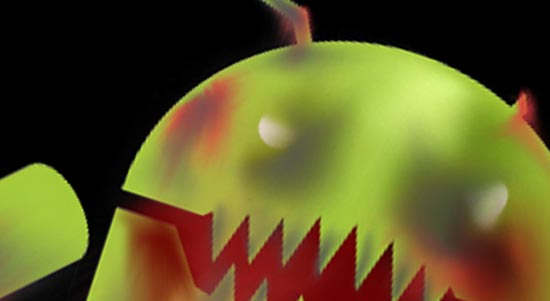
\includegraphics[height=\paperheight]{images/androidmalware.jpg}}
\begin{frame}

\mybox{Malware found...}
\footnotetext{\color{white}Image (CC BY 2.0) from: https://flic.kr/p/cuZZUY}
\end{frame}
}


\section{How we fucked up}

\begin{frame}
\frametitle{Meanwhile...}
\begin{dialogue}
\speak{Sebastian} Okay, weekend starts soon so I better remove that thing from the device so we can send it back...

\speak{Tibor} I will start analysis of the sample then and write the report.

\speak{Sebastian} Do you need anything from the device before I remove the malware?

\speak{Tibor} I don't think so...
\end{dialogue}
\end{frame}


\begin{frame}
\frametitle{Removal...}
\textit{Live Demo here... hopefully}
\end{frame}


{
\usebackgroundtemplate{
\includegraphics[height=\paperheight]{images/fuuu.jpg}}
\begin{frame}[plain]
%\mybox{FFFFFUUUUU!!!}
\end{frame}
}

\section{Shock!}

\section{Ideas}

\section{Recovery}

\section{Reversing}

\section{Learning}

\end{document}